
\renewcommand{\thechapter}{4}
\chapter{Denoising Theory}

As has been discussed, the performance of double-beta experiments like EXO-200 is partially determined by their energy resolution.  In EXO-200, the energy resolution is limited by the scintillation energy resolution, which in turn is dominated by electronic noise in the APDs.  Significant effort must therefore be expended to understand and reduce the noise in the scintillation signals.

\begin{figure}
\begin{center}
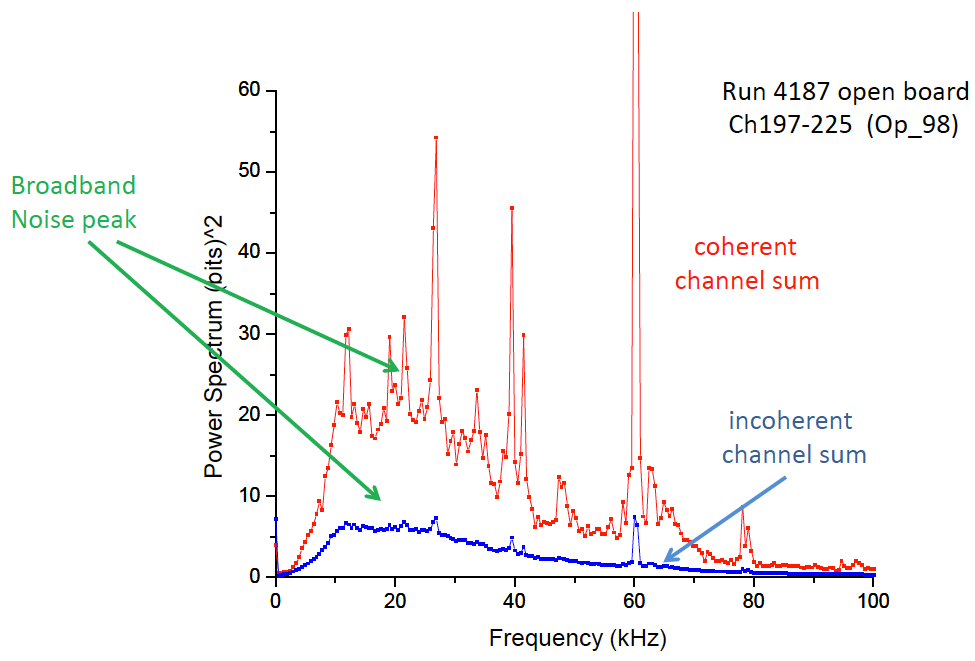
\includegraphics[keepaspectratio=true,width=\textwidth]{APDNoisePowerSpectrum.png}
\end{center}
\renewcommand{\baselinestretch}{1}
\small\normalsize
\begin{quote}
\caption{Coherent and incoherent noise power spectra for a sample set of APD channels without signal shaping.~\cite{ElectronicsUpgradeReport}}
\label{fig:APDNoisePowerSpectrum}
\end{quote}
\end{figure}
\renewcommand{\baselinestretch}{2}
\small\normalsize

When the noise in the APDs is studied, it was found that the individual APD channels met targetted root-mean-square noise levels of 2000 electrons.  However, rather than observing the noise on summed APD channels increase proportionally to the square root of the number of channels, the summed APD noise is roughly two to three times higher than projected.  This worse-than-expected scaling of the noise with channels indicates that noise across different channels is correlated, and further analysis confirms that the bulk of the noise on an unshaped APD waveform is correlated with other channels, as shown in Figure~\ref{fig:APDNoisePowerSpectrum}.  There are many possible sources of coherent noise in the hardware, and reducing the amount of coherent noise is a topic for further research.~\cite{ElectronicsUpgradeReport}

However, the observation that coherent noise is the dominant source of noise in the APDs, and thus also the limiting factor in EXO-200's energy resolution, means that it should be possible to exploit these correlations and reduce the level of noise in offline analysis.  This chapter will describe a scheme to accomplish that goal and produce an optimal estimate of scintillation energy which takes noise correlations into account.

It is worth noting that in fact there are a number of different qualitative approaches to reducing the noise levels in the scintillation channel.  In casual terms, we will refer to "passive" approaches as those in which components of our signals are weighted more or less heavily based on their relative signal-to-noise content.  "Active" approaches, by contrast, will be classified as those which attempt to improve the signal-to-noise content of signal components.  We have identified the following three types of denoising:
\begin{description}
\item[Frequency weighting] \hfill \\
On a given channel signal, weight more heavily the frequency components which contain larger signal-to-noise ratio.  This passive denoising scheme requires knowledge of the shapes in fourier space of a signal and the power spectrum of the noise.

\item[Channel weighting] \hfill \\
Different channels may have different levels of noise, so some may generally have higher-quality signals.  More importantly, though, the amount of signal on a given channel depends strongly on the proximity of the APD gang to the source of scintillation within the detector.  This passive denoising scheme therefore allows us to weight more heavily the channels which have more scintillation, provided we can identify these weights on an event-by-event basis.  This requires knowledge of the magnitude of noise on each channel and of the correspondence between event position and signal magnitude on each APD gang; the latter is described by the lightmap, described earlier.

\item[Noise subtraction] \hfill \\
This active form of denoising consists of using correlations between noise on different channels to produce a better estimate of the noise component of signals than each signal taken independently could provide.  To accomplish this, we will require detailed information about the pairwise noise correlations across channels at each frequency.
\end{description}

In the following, we will describe a general linear operator on the APD signals which in principle can accomplish each of these forms of denoising, and we will presume that all of the described inputs are available; by identifying the parameters for that linear operator which are optimal, we can be confident that the denoising operator we produce will accomplish all three forms of denoising described above.

\section{Setup}

We first establish a number of notational conventions:
\begin{itemize}
\item $i$, $j$ will represent indices over APD channels.
\item $t$ will represent the time indices of a discrete waveform.
\item $f$, $g$ will represent the frequency indices of Fourier-transformed waveforms.
\item $a$, $b$, $c$ will represent indices of signals in an event.
\item For a waveform $*[t]$, we will represent the discrete Fourier transform of that waveform with $\widetilde{*}[f]$, where the particular convention used to evaluate the Fourier transform is not significant.
\item For a Fourier-transformed waveform $\widetilde{*}[f]$, we denote the real and imaginary parts of that waveform by $\widetilde{*}^R[f]$ and $\widetilde{*}^I[f]$, respectively.
\item For an unknown parameter $*$, the symbol $\widehat{*}$ will identify an estimator for $*$.
\item For an expression $*$ containing random variables, $\left<*\right>$ is the expectation value of $*$.
\end{itemize}

We describe the data as a collection of discretely sampled waveforms, $X_i[t]$.  We assume that all signal times and shapes are already known, so we can model the waveforms by $X_i[t] = \sum_a M_{ia}Y_{ia}[t] + N_i[t] + b_i$, where $Y$ is the shape of signal $a$ on channel $i$, $M$ is the magnitude of that signal, and $N$ and $b$ represent the electronic noise and baseline, respectively, of the channel.

To break the degeneracy between $M$ and $Y$, we choose to fix the magnitude of the template signal $Y$.  We choose to require that the signal $Y$ has a magnitude of one, as described in figure~\ref{fig:SampleAPDTemplates}.  This implies that for a typical single-site $2615$-keV deposit, the average values of $M_i$ should be equal to the values of the lightmap $L_i(x,y,z,t)$ described earlier.

Noise correlations will be much simpler in frequency space, so we take the Fourier transform and drop the zero-frequency component to obtain \[\widetilde{X}_i[f] = \sum_a M_{ia}\widetilde{Y}_{ia}[f] + \widetilde{N}_i[f].\]

\section{The Signal Model}

It is first important to characterize the response of the APDs to energy deposits in EXO-200.  This will require us to understand the signal amplification of the detector at each physical stage, as well as the noise introduced by each of these processes.  We will describe both in detail here.

\subsection{APD Noise}

We will assume that there are two sources of noise in this model.  First, the electronic noise $N_i[t]$ is assumed to be random.  We require that noise with different frequencies is uncorrelated:
\[\left< \widetilde{N}_i[f] \widetilde{N}_j[g] \right> = 0 \text{~when~} f \ne g.\]
The noise correlations $\left< \widetilde{N}_i[f] \widetilde{N}_j[f] \right>$ are assumed to be known; our means for measuring them are described [ELSEWHERE].

The second random variable will be the magnitude of the signal itself, $M_{ia}$.  When an energetic decay occurs in bulk of the detector, it will release some number of photons.  We will denote the number of photons released by signal $a$ by $P^{(0)}_a$, and this is the parameter we wish to measure.  However, the magnitude signal actually observed on APD channels number of photons actually collected by sensors is a random variable whose distribution depends on $P^{(0)}_a$, and we will now identify the chain of events which produce it.

First, each APD gang $i$ has some number $P^{(1)}_{ia}$ of photons which reach them.  The mean fraction of photons reaching a particular gang $i$ from position $(x,y,z)$, $f_i(x,y,z)$, is assumed to be known; however, the initial paths of the optical photons emitted from the source, their trajectories through the Xenon, and their success in reflecting off of teflon are all random, so we treat $P^{(1)}_{ia}$ as a Poisson-distributed random variable with mean $f_i(x,y,z)P^{(0)}_a$.  A typical deposit from a $\beta\beta 0\nu$ event may deposit $10-100$ photons on each APD gang [CHECK THIS NUMBER], depending strongly on the location of the deposit; thus, we find that the Poisson noise on a single APD channel may be quite significant.

Additionally, the number of photons reaching different gangs are not uncorrelated; since a photon which reaches gang $i$ cannot deposit on a different gang $j$, $P^{(1)}_{ia}$ and $P^{(1)}_{ja}$ are anticorrelated for different gangs $i \ne j$.  This process is described by a multinomial distribution.  Explicitly, we can identify the expectation values of a multinomial distribution:
\begin{itemize}
\item $\left< P^{(1)}_{ia} \right> = f_i(x,y,z)P^{(0)}_a$
\item $\left< P^{(1)}_{ia} P^{(1)}_{jb} \right> = \left< P^{(1)}_{ia} \right> \left< P^{(1)}_{jb} \right> + \left[ f_i(x,y,z)\delta_{ij} - f_i(x,y,z)f_j(x,y,z) \right] P^{(0)}_a \delta_{ab}$
\end{itemize}

Following the random process associated with photons reaching the APD gangs, there is also randomness associated with signal amplification internally in the APDs.  These processes are described in detail in~\cite{EXOLAAPD}, but we can summarize that:

\begin{enumerate}
\item Optical photons in the liquid xenon arrive at the active layer of the APDs have a wavelength of roughly $178$ nm, meaning that each optical photon has an energy of roughly $7.0$ eV.  The energy required to produce one electron-hole pair in silicon is roughly $3.66$ eV, which means that each incident photon produces roughly $1.9$ electron-hole pairs; we will define $P^{(2)}_{ia}$ to be the number of electron-hole pairs actually produced from $P^{(1)}_{ia}$ incident photons.  The corresponding Fano factor for electrons produced in silicon is roughly $0.1$, meaning that in addition to the uncertainty in $P^{(1)}_{ia}$ which we have already characterized, there is an additional uncorrelated variance in $P^{(2)}_{ia}$ equal to $0.1 \left<P^{(2)}_{ia}\right>$.  The correlations in the parameters $P^{(2)}_{ia}$ are therefore:
\[\left< P^{(2)}_{ia} \right> = 1.9 \cdot P^{(1)}_{ia}\]
\[\left< P^{(2)}_{ia} P^{(2)}_{jb} \right> = (1.9)^2\left< P^{(1)}_{ia} P^{(1)}_{jb} \right> + 0.1 \left< P^{(2)}_{ia}\right> \delta_{ij}\delta_{ab}\]
\item Electron-hole pairs are then amplified by an avalanche process inside the APDs.  The magnitude of this gain is APD-dependent, generally on the order of $200-300$, and can be identified by a time-dependent quantity $G^P_i(t)$; we will call the number of output electrons $P^{(3)}_{ia}$.  In addition to amplification of existing noise in $P^{(2)}_{ia}$, two additional source of noise are introduced.  First, there is statistical variance in the amplification experienced by each electron due to the randomness of the avalanche process.  This variance is dependent on many factors, including the gain, and scales like the square root of the number of electrons; we define the variance on the gain experienced by a single electron as $\sigma^2_{G_i}(t)$.  Second, there are gain non-uniformities in the diode volume, which contribute variance proportional to the square of the number of initial electron-hole pairs; we will identify the proportionality constant as $\sigma^2_{NU}$, which may depend on time and APD gang.  The magnitude of this uncertainty is not well-known, but may be significant.  The correlations in the parameters $P^{(3)}_{ia}$ are therefore:
\[\left< P^{(3)}_{ia} \right> = G^P_i(t)P^{(2)}_{ia}\]
\[\left< P^{(3)}_{ia} P^{(3)}_{jb} \right> = G^P_i(t)G^P_j(t) \left< P^{(2)}_{ia} P^{(2)}_{jb} \right> + \left[P^{(2)}_{ia}\sigma^2_{G_i}(t) + \left(P^{(2)}_{ia}\right)^2\sigma^2_{NU}\right]\delta_{ij}\delta_{ab}\]
\end{enumerate}

Finally, there is amplification $G^{E}_i(t)$ associated with the electronics of the APDs which is dependent on time and channel.  This includes preamplifier gain, shaper gain, gain associated with the shaping times, and conversion from voltage to ADC counts.  We assume that no signal-dependent noise is introduced during this stage, but there is constant electronic noise $N_i[t]$ which has been described above.  Additionally, the APDs can contribute noise in the form of a dark current which is uncorrelated with signals; this is inseparable from the electronic noise, and so we absorb it into our description of $N_i[t]$.  Our final description of the signal magnitudes.

\subsection{APD Signals and Noise}

We have already characterized the overall gain of the APDs using the lightmap described earlier.  We know that a typical single-site deposit of $2615$ keV at position $(x,y,z)$ and time $t$ will produce a signal with expected magnitude $L_i(x,y,z,t)$ on APD channel $i$.  We must now connect this empirical understanding of our APD signals with the physical understanding in terms of photons and electrons described above.

We have identified the number of photons created by an event $a$ as $P^{(0)}_a$.  In reality, an ideal scintillation measurement can only measure this quantity, and not the true energy of the event -- there is randomness in the number of photons produced by a known-energy deposit, so $P^{(0)}_a$ will not be perfectly correlated with the energy $E_a$ of the event.  However, the number of photons generated is a difficult parameter to understand empirically, and all of our calibrations occur at a known energy even though the corresponding number of deposited photons is unknown.

Simulations using NEST~\cite{NESTpaper} which have been performed within the EXO group by Liangjian Wen at our bulk electric field indicate that we can expect roughly $82,000$ photons from a $2615$-keV gamma deposit.  We will identify this parameter with $c$, and express the average relation between energy and photon yield in EXO-200 by
$P^{(0)} = c \cdot E$,
where $E$ is the energy measured in units of $2615$ keV.  We will treat this relationship as exact, and attempt to measure $E$ rather than $P^{(0)}$; this means that when we speak of measuring the energy of an event using the APD signals, we really are referring to measuring the "scintillation energy," or a parameter proportional to the number of emitted photons which on average will equal the true energy of the deposit.

Ignoring variances for a moment, we can combine all of the expectation values for numbers of photons or ADC counts above to state that on average,
\[M_{ia} = 1.9 \cdot c f_i(x,y,z) G^P_i(t) G^E_i(t) E_a.\]
We can compare this to our empirical lightmap measurements, which are expressed by $M_{ia} = L_i(x,y,z,t) E_a$,
and we conclude that:
\[ L_i(x,y,z,t) = 1.9 \cdot c f_i(x,y,z) G^P_i(t) G^E_i(t).\]

We recall that it is assumed the lightmap is a separable function, $L_i(x,y,z,t) = R_i(x,y,z)S_i(t)$, and we can provide the two proportionalities:
\[ R_i(x,y,z) \propto f_i(x,y,z) \]
\[ S_i(t) \propto G^P_i(t) G^E_i(t).\]

Although $G^E_i(t)$ is in principle time-dependent, due to environmental effects on the APD electronics and occasional replacement of electronics cards for certain channels, precision data on its value is not readily available.  Instead, we use a time-independent estimate $G^E_i(t) = 1.1e-3$ ADC counts per electron emitted from the APD; the uncertainty in this figure is dominated by uncertainty in the preamplifier gains, which are controlled by a roughly $5$ pF capacitor.  Other contributors to the gain include shaper gain of $21.2$ (from a combination of amplification and shaping) and a full-scale digitizer range of $2.5$ volts for $12$-bit digitization.

We do have independent measurements of the APD gains $G^P_i(t)$ available from laser calibration runs.  These special runs allow a laser to shine into the detector from a fixed point and with a stable amplitude while the bias voltages on the APDs are varied from an effective unity gain to our standard voltage settings.  Using these measurements, we are able to measure $G^P_i(t)$ at weekly intervals from September 2012 to the present time.  Before September 2012, some less-reliable laser data is available, but results from that data are not readily available as of this writing.

It would be possible, and should be a goal for future improvements, to make use of this full range of laser data.  However, the laser data provides a less uniform history of APD gains over the full data-taking window of EXO-200 from September 2011 to November 2013, and it is much easier to track time-dependent behavior from Thorium source data which have been collected regularly throughout that period.  As a result, a compromise is used to characterize $G^P_i(t)$.  One particular laser run, run 4540 (taken on December 13, 2012), is used to fix $G^P_i(t_{4540})$, and the function is extrapolated using Thorium source data with:
\[G^P_i(t) \approx G^P_i(t_{4540}) \cdot S_i(t)/S_i(t_{4540}).\]
This assumption makes use of the approximation that $G^E_i(t)$ is roughly constant in time, which is probably only accurate to one significant figure; therefore when an electronics change is made to a channel, we can expect that the accuracy of $G^P_i(t)$ is no better than one significant figure.  These results mean that we can also estimate with the same level of accuracy:
\[f_i(x,y,z) \approx \frac{S_i(t_{4540})}{G^P_i(t_{4540})} \cdot \frac{R_i(x,y,z)}{1.9 \cdot c G^E_i(t)}.\]

It is then possible to express the full correlations in signal magnitudes in terms of the scintillation energies of deposits as:
\begin{align*}
\left< M_{ia} \right> &= L_i(x,y,z,t) E_a \\
\begin{split}
\left< M_{ia} M_{jb} \right> &= L_i(x,y,z,t)L_j(x,y,z,t) E_a E_b \left[1 + \frac{\sigma^2_{NU}}{\left(G^P_i(t)\right)^2} \delta_{ij}\delta_{ab} \right] \\
&\quad - L_i(x,y,z,t) L_j(x,y,z,t) E_a \delta_{ab}/c \\
&\quad + L_i(x,y,z,t) G^E_i(t) E_a \delta_{ij} \delta_{ab} \left[\left(0.1 + 1.9\right)G^P_i(t) + \frac{\sigma^2_{G_i}(t)}{G^P_i(t)}\right].
\end{split}\end{align*}
\begin{comment}
THE FOLLOWING IS MY WORK IN EXPANDING THE M_M CORRELATIONS.
IF NEEDED, IT CAN BE UNCOMMENTED AND IS VALID LATEX CODE.

\[ \left< M_{ia} M_{jb} \right> = G^E_i(t) G^E_j(t) \left<P^{(3)}_{ia}P^{(3)}_{jb} \right> \]

\[ \left< M_{ia} M_{jb} \right> = G^E_i(t) G^E_j(t) \left( G^P_i(t)G^P_j(t) \left< P^{(2)}_{ia} P^{(2)}_{jb} \right> + \left[P^{(2)}_{ia}\sigma^2_{G_i}(t) + \left(P^{(2)}_{ia}\right)^2\sigma^2_{NU}\right]\delta_{ij}\delta_{ab}\right)\]

\begin{equation*}\begin{split}
\left< M_{ia} M_{jb} \right> ={}& G^E_i(t) G^E_j(t) G^P_i(t)G^P_j(t) \left< P^{(2)}_{ia} P^{(2)}_{jb} \right> \\
 & + G^E_i(t) G^E_j(t) \left[P^{(2)}_{ia}\sigma^2_{G_i}(t) + \left(P^{(2)}_{ia}\right)^2\sigma^2_{NU}\right]\delta_{ij}\delta_{ab}
\end{split}\end{equation*}

\begin{equation*}\begin{split}
\left< M_{ia} M_{jb} \right> ={}& G^E_i(t) G^E_j(t) G^P_i(t)G^P_j(t) \left( (1.9)^2\left< P^{(1)}_{ia} P^{(1)}_{jb} \right> + 0.1 \left< P^{(2)}_{ia}\right> \delta_{ij}\delta_{ab} \right) \\
 & + G^E_i(t) G^E_j(t) \left[1.9 \cdot P^{(1)}_{ia}\sigma^2_{G_i}(t) + (1.9)^2 \left(P^{(1)}_{ia}\right)^2\sigma^2_{NU}\right]\delta_{ij}\delta_{ab}
\end{split}\end{equation*}

\begin{equation*}\begin{split}
\left< M_{ia} M_{jb} \right> ={}& (1.9)^2 G^E_i(t) G^E_j(t) G^P_i(t)G^P_j(t) \left< P^{(1)}_{ia} P^{(1)}_{jb} \right> \\
& + 0.1 \cdot 1.9 \cdot G^E_i(t) G^E_j(t) G^P_i(t)G^P_j(t) P^{(1)}_{ia} \delta_{ij}\delta_{ab} \\
 & + G^E_i(t) G^E_j(t) \left[1.9 \cdot P^{(1)}_{ia}\sigma^2_{G_i}(t) + (1.9)^2 \left(P^{(1)}_{ia}\right)^2\sigma^2_{NU}\right]\delta_{ij}\delta_{ab}
\end{split}\end{equation*}

\begin{equation*}\begin{split}
\left< M_{ia} M_{jb} \right> ={}& (1.9)^2 G^E_i(t) G^E_j(t) G^P_i(t)G^P_j(t) \left< P^{(1)}_{ia} P^{(1)}_{jb} \right> \\
 & + G^E_i(t) G^E_j(t) \left[1.9 \cdot P^{(1)}_{ia}\sigma^2_{G_i}(t) + (1.9)^2 \left(P^{(1)}_{ia}\right)^2\sigma^2_{NU} + 0.1 \cdot 1.9 \cdot G^P_i(t)G^P_j(t) P^{(1)}_{ia}\right]\delta_{ij}\delta_{ab}
\end{split}\end{equation*}

\begin{equation*}\begin{split}
\left< M_{ia} M_{jb} \right> ={}& (1.9)^2 G^E_i(t) G^E_j(t) G^P_i(t)G^P_j(t) \left< P^{(1)}_{ia} P^{(1)}_{jb} \right> \\
 & + 1.9\left[\sigma^2_{G_i}(t) + 1.9 \cdot P^{(1)}_{ia} \sigma^2_{NU} + 0.1 \cdot G^P_i(t)G^P_j(t) \right] \left(G^E_i(t)\right)^2 P^{(1)}_{ia} \delta_{ij}\delta_{ab}
\end{split}\end{equation*}

\begin{equation*}\begin{split}
\left< M_{ia} M_{jb} \right> ={}& (1.9)^2 G^E_i(t) G^E_j(t) G^P_i(t)G^P_j(t) \left< P^{(1)}_{ia} \right> \left< P^{(1)}_{jb} \right> \\
& + (1.9)^2 G^E_i(t) G^E_j(t) G^P_i(t)G^P_j(t)\left[ f_i(x,y,z)\delta_{ij} - f_i(x,y,z)f_j(x,y,z) \right] P^{(0)}_a \delta_{ab}  \\
 & + 1.9\left[\sigma^2_{G_i}(t) + 1.9 \cdot P^{(1)}_{ia} \sigma^2_{NU} + 0.1 \cdot G^P_i(t)G^P_j(t) \right] \left(G^E_i(t)\right)^2 P^{(1)}_{ia} \delta_{ij}\delta_{ab}
\end{split}\end{equation*}

\begin{equation*}\begin{split}
\left< M_{ia} M_{jb} \right> ={}& (1.9)^2 G^E_i(t) G^E_j(t) G^P_i(t)G^P_j(t) f_i(x,y,z) f_j(x,y,z) \left(P^{(0)}_a\right)^2 \\
& + (1.9)^2 G^E_i(t) G^E_j(t) G^P_i(t)G^P_j(t)\left[ f_i(x,y,z)\delta_{ij} - f_i(x,y,z)f_j(x,y,z) \right] P^{(0)}_a \delta_{ab}  \\
 & + 1.9\left[\sigma^2_{G_i}(t) + 1.9 \cdot f_i(x,y,z) P^{(0)}_a \sigma^2_{NU} + 0.1 \cdot G^P_i(t)G^P_j(t) \right] \left(G^E_i(t)\right)^2 f_i(x,y,z) P^{(0)}_a \delta_{ij}\delta_{ab}
\end{split}\end{equation*}

\begin{equation*}\begin{split}
\left< M_{ia} M_{jb} \right> ={}& (1.9)^2 G^E_i(t) G^E_j(t) G^P_i(t)G^P_j(t) f_i(x,y,z) f_j(x,y,z) c^2 E^2_a \\
& + (1.9)^2 G^E_i(t) G^E_j(t) G^P_i(t)G^P_j(t)\left[ f_i(x,y,z)\delta_{ij} - f_i(x,y,z)f_j(x,y,z) \right] c E_a \delta_{ab}  \\
 & + 1.9\left[\sigma^2_{G_i}(t) + 1.9 \cdot f_i(x,y,z) c E_a \sigma^2_{NU} + 0.1 \cdot G^P_i(t)G^P_j(t) \right] \left(G^E_i(t)\right)^2 f_i(x,y,z) c E_a \delta_{ij}\delta_{ab}
\end{split}\end{equation*}

\begin{equation*}\begin{split}
\left< M_{ia} M_{jb} \right> ={}& L_i(x,y,z,t)L_j(x,y,z,t) E^2_a \\
& + (1.9)^2 G^E_i(t) G^E_j(t) G^P_i(t)G^P_j(t) f_i(x,y,z)\delta_{ij} c E_a \delta_{ab}  \\
& - (1.9)^2 G^E_i(t) G^E_j(t) G^P_i(t)G^P_j(t) f_i(x,y,z)f_j(x,y,z) c E_a \delta_{ab} \\
 & + 1.9\left[\sigma^2_{G_i}(t) + 1.9 \cdot f_i(x,y,z) c E_a \sigma^2_{NU} + 0.1 \cdot G^P_i(t)G^P_j(t) \right] \left(G^E_i(t)\right)^2 f_i(x,y,z) c E_a \delta_{ij}\delta_{ab}
\end{split}\end{equation*}

\begin{equation*}\begin{split}
\left< M_{ia} M_{jb} \right> ={}& L_i(x,y,z,t)L_j(x,y,z,t) E^2_a \\
& + L_i(x,y,z,t) (1.9)  G^E_i(t) G^P_i(t) \delta_{ij}  E_a \delta_{ab}  \\
& - L_i(x,y,z,t)     (1.9) G^E_j(t) G^P_j(t) f_j(x,y,z) E_a \delta_{ab} \\
 & + 1.9\left[\sigma^2_{G_i}(t) + 1.9 \cdot f_i(x,y,z) c E_a \sigma^2_{NU} + 0.1 \cdot \left(G^P_i(t)\right)^2 \right] \left(G^E_i(t)\right)^2 f_i(x,y,z) c E_a \delta_{ij}\delta_{ab}
\end{split}\end{equation*}

\begin{equation*}\begin{split}
\left< M_{ia} M_{jb} \right> ={}& L_i(x,y,z,t)L_j(x,y,z,t) E^2_a \\
& + L_i(x,y,z,t) (1.9)  G^E_i(t) G^P_i(t) E_a \delta_{ij} \delta_{ab}  \\
& - L_i(x,y,z,t) L_j(x,y,z,t) E_a \delta_{ab}/c \\
& + (1.9)\sigma^2_{G_i}(t)\left(G^E_i(t)\right)^2 f_i(x,y,z) c E_a \delta_{ij}\delta_{ab} \\
& + (1.9)^2 f_i(x,y,z) c E_a \sigma^2_{NU} \left(G^E_i(t)\right)^2 f_i(x,y,z) c E_a \delta_{ij}\delta_{ab} \\
& + (1.9) (0.1) \left(G^P_i(t)\right)^2 \left(G^E_i(t)\right)^2 f_i(x,y,z) c E_a \delta_{ij}\delta_{ab}
\end{split}\end{equation*}

\begin{equation*}\begin{split}
\left< M_{ia} M_{jb} \right> ={}& L_i(x,y,z,t)L_j(x,y,z,t) E^2_a \\
& + (1.9)^2 f^2_i(x,y,z) \sigma^2_{NU} \left(G^E_i(t)\right)^2 c^2 E^2_a \delta_{ij}\delta_{ab} \\
& - L_i(x,y,z,t) L_j(x,y,z,t) E_a \delta_{ab}/c \\
& + L_i(x,y,z,t) (1.9)  G^E_i(t) G^P_i(t) E_a \delta_{ij} \delta_{ab}  \\
& + (1.9)\sigma^2_{G_i}(t)\left(G^E_i(t)\right)^2 f_i(x,y,z) c E_a \delta_{ij}\delta_{ab} \\
& + L_i(x,y,z,t) (0.1) G^P_i(t) G^E_i(t) E_a \delta_{ij}\delta_{ab}
\end{split}\end{equation*}

\begin{equation*}\begin{split}
\left< M_{ia} M_{jb} \right> ={}& L_i(x,y,z,t)L_j(x,y,z,t) E^2_a \\
& + L^2_i(x,y,z,t) \sigma^2_{NU} E^2_a \delta_{ij}\delta_{ab}/\left(G^P_i(t)\right)^2 \\
& - L_i(x,y,z,t) L_j(x,y,z,t) E_a \delta_{ab}/c \\
& + L_i(x,y,z,t) (1.9)  G^E_i(t) G^P_i(t) E_a \delta_{ij} \delta_{ab}  \\
& + L_i(x,y,z,t) \sigma^2_{G_i}(t)G^E_i(t) E_a \delta_{ij}\delta_{ab}/G^P_i(t) \\
& + L_i(x,y,z,t) (0.1) G^P_i(t) G^E_i(t) E_a \delta_{ij}\delta_{ab}
\end{split}\end{equation*}

\begin{equation*}\begin{split}
\left< M_{ia} M_{jb} \right> ={}& L_i(x,y,z,t)L_j(x,y,z,t) E^2_a \left[1 + \frac{\sigma^2_{NU}}{\left(G^P_i(t)\right)^2} \delta_{ij}\delta_{ab} \right] \\
& - L_i(x,y,z,t) L_j(x,y,z,t) E_a \delta_{ab}/c \\
& + L_i(x,y,z,t) \sigma^2_{G_i}(t)G^E_i(t) E_a \delta_{ij}\delta_{ab}/G^P_i(t) \\
& + L_i(x,y,z,t) (1.9 + 0.1)  G^E_i(t) G^P_i(t) E_a \delta_{ij} \delta_{ab}
\end{split}\end{equation*}

\begin{equation*}\begin{split}
\left< M_{ia} M_{jb} \right> ={}& L_i(x,y,z,t)L_j(x,y,z,t) E^2_a \left[1 + \frac{\sigma^2_{NU}}{\left(G^P_i(t)\right)^2} \delta_{ij}\delta_{ab} \right] \\
& - L_i(x,y,z,t) L_j(x,y,z,t) E_a \delta_{ab}/c \\
& + L_i(x,y,z,t) G^E_i(t) E_a \delta_{ij} \delta_{ab} \left[\left(0.1 + 1.9\right)G^P_i(t) + \frac{\sigma^2_{G_i}(t)}{G^P_i(t)}\right]
\end{split}\end{equation*}
\end{comment}

We combine this with our knowledge of the noise coefficients:
\begin{align*}
\left< \widetilde{N}_i[f] \right> &= 0 \\
\left< \widetilde{N}_i[f] \widetilde{N}_j[g] \right> &= \left\{ \begin{aligned}
0~ &\text{if}~ f \ne g \\
\text{known}~ &\text{if}~ f = g
\end{aligned}\right.
\end{align*}
and can claim to now have a complete description of the signals and noise observed in the APD channels.

\section{Derivation}

It is now possible to specify the optimization criteria for generating an energy estimate from the APD signals.  We wish to identify an energy estimator which is unbiased and has a minimal expected error.  For the problem to remain tractable, we will demand that the operator be linear.  Furthermore, although the Fourier-transformed waveforms $\widetilde{X}_i[f]$ are complex-valued, we will require that the energy estimate be strictly real-valued.

We will therefore take the energy estimator to be of the form:
\[ \widehat{E}_a = \sum_{if} A_{ifa} \widetilde{X}_i^R[f] + B_{ifa} \widetilde{X}_i^I[f].\]
The goal of denoising is therefore reduced to identifying the optimal parameters $A_{ifa}$ and $B_{ifa}$ for this estimator.

The error in the energy estimate $\widehat{E}_a$ of $E_a$ is defined by:
\[ \epsilon^2_a = \left< \left(\widehat{E}_a - E_a\right)^2\right>. \]
Our goal is then to minimize $\epsilon^2_a$ under the constraint of no bias, ie. that:
\[\left<\widehat{E}_a - E_a\right> = 0\]
or, equivalently,
\[\sum_{ifb}\left[A_{ifa} \widetilde{Y}_{ib}^R[f] + B_{ifa} \widetilde{Y}_{ib}^I[f]\right] L_i(x,y,z,t) E_b = E_a.\]
However, we will find that it is necessary to specify a slightly stronger constraint.  In particular, it will be desirable to ensure that the constraints are as independent of energy as possible to reduce the need to input an estimated energy into our energy estimator; therefore we will freely employ the stronger constraint
\[\sum_{if}\left[A_{ifa} \widetilde{Y}_{ib}^R[f] + B_{ifa} \widetilde{Y}_{ib}^I[f]\right] L_i(x,y,z,t) = \delta_{ab}\]
which implies the earlier forms and leads to advantageous cancellations of terms.

We now proceed with the optimization.  We start by expanding $\epsilon^2_a$:
\begin{align*}
\epsilon^2_a &= \left< \left(\widehat{E}_a - E_a\right)^2\right> \\
%
&= \left< \widehat{E}^2_a \right> - E_a \left<\widehat{E}_a\right> - \left< \widehat{E}_a - E_a \right> E_a \\
%
\intertext{We can employ the constraint to simplify the second term of this expansion, and eliminate the third altogether; we then proceed:}
%
&= \left< \widehat{E}^2_a \right> - E^2_a \\
%
&= \left< \left(\sum_{if}\left[ A_{ifa} \widetilde{X}_i^R[f] + B_{ifa} \widetilde{X}_i^I[f]\right]\right)^2\right> - E^2_a \\
%
& \begin{aligned}= \bigg< \bigg(&
  \sum_{if} \left[ A_{ifa} \widetilde{N}_i^R[f] + B_{ifa} \widetilde{N}_i^I[f]\right] \\
  & + \sum_{ifb} \left[ A_{ifa} \widetilde{Y}_{ib}^R[f] + B_{ifa} \widetilde{Y}_{ib}^I[f]\right]M_{ib}  \bigg)^2 \bigg> - E^2_a
\end{aligned} \\
%
\intertext{The noise $\widetilde{N}$ and signal $M_{ia}$ are uncorrelated, so multiplicative cross-terms will have an expectation value of zero:}
%
&= \left< \left(\sum_{if} \left[ A_{ifa} \widetilde{N}_i^R[f] + B_{ifa} \widetilde{N}_i^I[f]\right]\right)^2\right> \\
&\quad + \left<\left(\sum_{ifb} \left[ A_{ifa} \widetilde{Y}_{ib}^R[f] + B_{ifa} \widetilde{Y}_{ib}^I[f]\right]M_{ib} \right)^2 \right> - E^2_a \\
%
\intertext{Additionally, only electronic noise cross-terms between different frequencies will not survive:}
%
&= \left< \sum_{ijf} \left[ A_{ifa} \widetilde{N}_i^R[f] + B_{ifa} \widetilde{N}_i^I[f]\right] \left[ A_{jfa} \widetilde{N}_j^R[f] + B_{jfa} \widetilde{N}_j^I[f]\right] \right> \\
&\quad + \left<\left(\sum_{ifb} \left[ A_{ifa} \widetilde{Y}_{ib}^R[f] + B_{ifa} \widetilde{Y}_{ib}^I[f]\right]M_{ib} \right)^2 \right> - E^2_a \\
%
& \begin{aligned}
  = \sum_{ijf} \bigg[ & A_{ifa}A_{jfa} \left<\widetilde{N}_i^R[f]\widetilde{N}_j^R[f]\right> + A_{ifa}B_{jfa} \left<\widetilde{N}_i^R[f]\widetilde{N}_j^I[f]\right> \\
  & + B_{ifa}A_{jfa} \left<\widetilde{N}_i^I[f]\widetilde{N}_j^R[f]\right> + B_{ifa}B_{jfa} \left<\widetilde{N}_i^I[f]\widetilde{N}_j^I[f]\right>\bigg] \end{aligned} \\
&\quad + \sum_{\substack{ifb\\jgc}} \left[A_{ifa} \widetilde{Y}_{ib}^R[f] + B_{ifa} \widetilde{Y}_{ib}^I[f]\right]\left[A_{jga} \widetilde{Y}_{jc}^R[g] + B_{jga} \widetilde{Y}_{jc}^I[g]\right] \left<M_{ib}M_{jc}\right> - E^2_a \\
%
\intertext{We will now expand $\left<M_{ib}M_{jc}\right>$ and take advantage of the stronger form of our constraint to simplify the expression:}
%
& \begin{aligned}
  = \sum_{ijf} \bigg[ & A_{ifa}A_{jfa} \left<\widetilde{N}_i^R[f]\widetilde{N}_j^R[f]\right> + A_{ifa}B_{jfa} \left<\widetilde{N}_i^R[f]\widetilde{N}_j^I[f]\right> \\
  & + B_{ifa}A_{jfa} \left<\widetilde{N}_i^I[f]\widetilde{N}_j^R[f]\right> + B_{ifa}B_{jfa} \left<\widetilde{N}_i^I[f]\widetilde{N}_j^I[f]\right>\bigg] \end{aligned} \\
&\quad + \left( \sum_{ifb} \left[A_{ifa} \widetilde{Y}_{ib}^R[f] + B_{ifa} \widetilde{Y}_{ib}^I[f]\right] L_i(x,y,z,t) E_b \right)^2 - E^2_a \\
&\quad - \sum_b \left( \sum_{if} \left[A_{ifa} \widetilde{Y}_{ib}^R[f] + B_{ifa} \widetilde{Y}_{ib}^I[f]\right] L_i(x,y,z,t) \right)^2 \frac{E_b}{c} \\
&\quad \begin{aligned}
  + \sum_{ifgb} &\left[A_{ifa} \widetilde{Y}_{ib}^R[f] + B_{ifa} \widetilde{Y}_{ib}^I[f]\right]\left[A_{iga} \widetilde{Y}_{ib}^R[g] + B_{iga} \widetilde{Y}_{ib}^I[g]\right] \cdot \\
  & \begin{aligned}
    L_i(x,y,z,t) E_b \bigg[ &(0.1 + 1.9) G^E_i(t) G^P_i(t) \\
    & + \frac{G^E_i(t)}{G^P_i(t)} \sigma^2_{G_i}(t) + L_i(x,y,z,t) E_b \frac{\sigma^2_{NU}}{\left(G^P_i(t)\right)^2} \bigg]
\end{aligned} \end{aligned} \\
%
& \begin{aligned}
  = \sum_{ijf} \bigg[ & A_{ifa}A_{jfa} \left<\widetilde{N}_i^R[f]\widetilde{N}_j^R[f]\right> + A_{ifa}B_{jfa} \left<\widetilde{N}_i^R[f]\widetilde{N}_j^I[f]\right> \\
  & + B_{ifa}A_{jfa} \left<\widetilde{N}_i^I[f]\widetilde{N}_j^R[f]\right> + B_{ifa}B_{jfa} \left<\widetilde{N}_i^I[f]\widetilde{N}_j^I[f]\right>\bigg] \end{aligned} \\
&\quad \begin{aligned}
  + \sum_{ifgb} &\left[A_{ifa} \widetilde{Y}_{ib}^R[f] + B_{ifa} \widetilde{Y}_{ib}^I[f]\right]\left[A_{iga} \widetilde{Y}_{ib}^R[g] + B_{iga} \widetilde{Y}_{ib}^I[g]\right] \cdot \\
  & \begin{aligned}
    L_i(x,y,z,t) E_b \bigg[ &(0.1 + 1.9) G^E_i(t) G^P_i(t) \\
    & + \frac{G^E_i(t)}{G^P_i(t)} \sigma^2_{G_i}(t) + L_i(x,y,z,t) E_b \frac{\sigma^2_{NU}}{\left(G^P_i(t)\right)^2} \bigg]
\end{aligned} \end{aligned} \\
&\quad - \frac{E_a}{c}
\end{align*}

We are now in a position to evaluate the partial derivatives of $\epsilon^2_a$ with respect to the parameters $A_{ifa}$ and $B_{ifa}$.  They are:
\begin{align*}
\frac{\partial \epsilon^2_a}{\partial A_{ifa}} &= 2 \sum_j \left[ A_{jfa} \left<\widetilde{N}_i^R[f]\widetilde{N}_j^R[f]\right> + B_{jfa} \left<\widetilde{N}_i^R[f]\widetilde{N}_j^I[f]\right>\right] \\
&\quad \begin{aligned}
  + 2 \sum_{gb} & E_b\widetilde{Y}_{ib}^R[f] L_i(x,y,z,t)\left[A_{jga} \widetilde{Y}_{jb}^R[g] + B_{jga} \widetilde{Y}_{jb}^I[g]\right] \cdot \\
  & \begin{aligned}
    \bigg[ &(0.1 + 1.9) G^E_i(t) G^P_i(t) \\
  & + \frac{G^E_i(t)}{G^P_i(t)} \sigma^2_{G_i}(t) + L_i(x,y,z,t) E_b \frac{\sigma^2_{NU}}{\left(G^P_i(t)\right)^2} \bigg]
\end{aligned} \end{aligned}\\
%
\frac{\partial \epsilon^2_a}{\partial B_{ifa}} &= 2 \sum_j \left[ A_{jfa} \left<\widetilde{N}_i^I[f]\widetilde{N}_j^R[f]\right> + B_{jfa} \left<\widetilde{N}_i^I[f]\widetilde{N}_j^I[f]\right>\right] \\
&\quad \begin{aligned}
  + 2 \sum_{gb} & E_b\widetilde{Y}_{ib}^I[f] L_i(x,y,z,t)\left[A_{jga} \widetilde{Y}_{jb}^R[g] + B_{jga} \widetilde{Y}_{jb}^I[g]\right] \cdot \\
  & \begin{aligned}
    \bigg[ &(0.1 + 1.9) G^E_i(t) G^P_i(t) \\
  & + \frac{G^E_i(t)}{G^P_i(t)} \sigma^2_{G_i}(t) + L_i(x,y,z,t) E_b \frac{\sigma^2_{NU}}{\left(G^P_i(t)\right)^2} \bigg]
\end{aligned} \end{aligned}
\end{align*}








\section{Preconditioning}

The matrix equation we wish to solve takes the form:
\[\begin{pmatrix}
E+P & L\\
L^\top & 0
\end{pmatrix}
X = 
\begin{pmatrix}
0 \\ I
\end{pmatrix}\]
Let us define $D = diag(E)$ and approximate
\[\begin{pmatrix}
E+P & L\\
L^\top & 0
\end{pmatrix}
\approx
\begin{pmatrix}
D & L\\
L^\top & 0
\end{pmatrix}\]
This approximate form is easy to invert, and can be used to precondition our problem for better numerical behavior.

We can further factor this approximate form of the matrix:
\[
\begin{array}{cccc}
\begin{pmatrix}
D & L\\
L^\top & 0
\end{pmatrix}
&=&
\begin{pmatrix}
D^{1/2} & 0\\
L^\top D^{-1/2} & -H^\top
\end{pmatrix}
&
\begin{pmatrix}
D^{1/2} & D^{-1/2}L\\
0 & H
\end{pmatrix}\\[1em]
&=&

\begin{pmatrix}
D^{1/2} & 0\\
0 & I
\end{pmatrix}
\begin{pmatrix}
I & 0\\
L^\top D^{-1/2} & -H^\top
\end{pmatrix}
&
\begin{pmatrix}
I & D^{-1/2}L\\
0 & H
\end{pmatrix}
\begin{pmatrix}
D^{1/2} & 0\\
0 & I
\end{pmatrix}

\end{array}
\]
where $H$ is defined uniquely by $H^\top H = L^\top D^{-1} L$.  (The solution is guaranteed to be real because D is positive-semidefinite -- it consists of noise variance terms, which are non-negative.)

The two diagonal factors are easily inverted; we further define
\[
\begin{array}{cc}
K_1 =
\begin{pmatrix}
I & 0\\
L^\top D^{-1/2} & -H^\top
\end{pmatrix}
&
K_1^{-1} =
\begin{pmatrix}
I & 0\\
{H^\top}^{-1}L^\top D^{-1/2} & -{H^\top}^{-1}
\end{pmatrix}\\
K_2 =
\begin{pmatrix}
I & D^{-1/2}L\\
0 & H
\end{pmatrix}
&
K_2^{-1} =
\begin{pmatrix}
I & -D^{-1/2}LH^{-1}\\
0 & H^{-1}
\end{pmatrix}
\end{array}
\]
and then follow the standard proscription for preconditioning a linear system:
\begin{gather*}
K_1^{-1} \begin{pmatrix}D^{-1/2}&0\\0&I\end{pmatrix}
\begin{pmatrix}
E+P & L\\
L^\top & 0
\end{pmatrix}
\begin{pmatrix}D^{-1/2}&0\\0&I\end{pmatrix} K_2^{-1} Z = 
K_1^{-1} \begin{pmatrix}D^{-1/2}&0\\0&I\end{pmatrix} \begin{pmatrix}0\\I\end{pmatrix}\\
Z = K_2 \begin{pmatrix}D^{1/2} & 0\\0 & I\end{pmatrix}X
\end{gather*}
which reduces to
\begin{gather*}
K_1^{-1} 
\left[
\begin{pmatrix}D^{-1/2}ED^{-1/2}&0\\0&0\end{pmatrix}
+
\begin{pmatrix}D^{-1/2}PD^{-1/2}&D^{-1/2}L\\L^\top D^{-1/2}&0\end{pmatrix}
\right]
K_2^{-1} Z = 
\begin{pmatrix}0\\-{H^\top}^{-1}\end{pmatrix}\\
X = \begin{pmatrix}D^{-1/2}&0\\0&I\end{pmatrix}K_2^{-1}Z
\end{gather*}

This preconditioned set of equations is numerically quite stable.  It is also possible to provide an excellent initial guess $Z_0$ by taking the approximate form of the matrix to be exact, yielding
\[
Z_0 = \begin{pmatrix}0\\-{H^\top}^{-1}\end{pmatrix}
\]
Based on these various advantages, it is this system which we attempt to solve rather than the original form.  Below we define matrices $A$ and $B$ for convenience, and summarize the system to be solved:
\[\begin{array}{rcl}
A &=& K_1^{-1} 
\left[
\begin{pmatrix}D^{-1/2}ED^{-1/2}&0\\0&0\end{pmatrix}
+
\begin{pmatrix}D^{-1/2}PD^{-1/2}&D^{-1/2}L\\L^\top D^{-1/2}&0\end{pmatrix}
\right]
K_2^{-1}\\
B &=& Z_0 = \begin{pmatrix}0\\-{H^\top}^{-1}\end{pmatrix}\\
AZ &=& B\\
X &=&  \begin{pmatrix}D^{-1/2}&0\\0&I\end{pmatrix}K_2^{-1}Z
\end{array}\]


\section{Solver}

The matrix $Z$ for which we attempt to solve will have as many columns as there are signals we wish to simultaneously refit within an event; in the case of light-only denoising and with the restriction that we only examine events with one scintillation signal, $Z$ will always have exactly one column.  In general, though, it may be desirable to denoise events with multiple scintillation signals; or it may be beneficial to denoise certain wire channels (which may include wire signals) simultaneously with the APD channels.  In these cases the number of columns may be larger -- five or six columns may not be unusual.  In such cases it would be possible to solve for each column of $Z$ independently, but more efficient to solve the entire system simultaneously.  In this way, information obtained from multiplying the matrix by one column may be exploited to solve the other columns as well, effectively multiplying the benefit from each matrix-multiplication by the number of columns of $Z$.\footnote{In practice the improvement is not quite so impressive, for two reasons: the vectors which are most useful toward solving one column may not be the most useful toward solving another; and some columns may achieve a solution earlier than others, yet are difficult to terminate without restarting the solver entirely.  These challenges have not appeared to be significant for this particular system.}

The algorithm which we have selected for solving this system is the block variant of the stabilized biconjugate-gradient method (Bl-BiCGSTAB) [CITE THIS].  It is reproduced here in the form used by our code.

\begin{algorithmic}
\STATE $R \gets B-AZ_0$
\STATE $P \gets R$
\STATE $\widetilde{R_0} \gets R$
\WHILE{any column of $R$ has a magnitude greater than desired}
  \STATE $V \gets AP$
  \STATE Solve $(\widetilde{R_0}^\top V)\alpha = (\widetilde{R_0}^\top R)$ for $\alpha$.
  \STATE $R \gets R - V\alpha$
  \STATE $T \gets AR$
  \STATE $\omega \gets {\langle T,S\rangle_F} / {\langle T,T\rangle_F} $
    \COMMENT{where $\langle\cdot,\cdot\rangle_F$ is the Frobenius matrix norm.}
  \STATE $Z \gets Z + P\alpha + \omega R$
  \STATE $R \gets R - \omega T$
  \STATE $R$ currently equals $B-AZ$; if it is small enough, terminate.
  \STATE Solve $(\widetilde{R_0}^\top V)\beta = -(\widetilde{R_0}^\top T)$ for $\beta$.
  \STATE $P \gets R + (P - \omega V) \beta$
\ENDWHILE

\end{algorithmic}

Since each column of $Z$ corresponds to one signal we are refitting, the norm of the corresponding column of $R$ tells us how well we have identified the optimal magnitude estimator for that signal; thus, to test for termination we should evaluate the norm of each column of $R$, and while any of those norms are above some threshold, the solver must be permitted to continue.  Because our resolution is only on the order of $1\%$, solutions generally need not be very accurate; in practice, we establish reasonable thresholds by plotting resolution against threshold for a small subset of data, and observing when the resolution stops improving.

\section{Implementation}

Although the previous section described the algorithm used for solving these matrix equations, in practice the processing time required is significant.  There are certain implementation tricks which can be applied with significant impact.  These are described here.

FILL-IN: Poisson multiplication using common factors.

After reducing the complexity of handling Poisson terms in this way, the handling of electronic noise terms in matrix multiplication becomes the computational bottleneck.  The structure of the problem is that the matrix containing electronic noise terms is block-diagonal; that is, it consists of one dense block per frequency component, with each block lying on the diagonal and where the number of rows and columns is twice the number of channels being denoised (except for the last frequency component, where imaginary terms are identically equal to zero).  The problem of handling electronic noise terms thus consists of $1024$ matrix-matrix multiplications, with the left matrix of approximate size $300\times300$ and the right matrix of approximate size $300\times O(1)$.\footnote{The number of columns in the right matrix is equal to the number of signals, which may be sometimes $3-5$ or more; however, it is always much smaller than $300$, and describing it as $O(1)$ captures this fact.}

The key points here which create an opportunity for optimization are that:
\begin{itemize}
\item The electronic noise terms generally do not change event-by-event.  They are treated as constant across many runs.
\item It is possible to multiply two $N \times N$ matrices together much faster than it is possible to perform $N$ multiplications of an $N \times N$ matrix with $N$ $N \times 1$ matrices.  This can be achieved with a combination of algorithms faster than naive $O(N^3)$ speed and exploitation of low-level computer hardware features such as the CPU cache. [Provide a citation!]
\end{itemize}
What we wish to do, then, is reorganize the solver algorithm so that whenever multiplication by the electronic noise matrix is required, rather than performing that multiplication on a ``skinny" $300 \times O(1)$ matrix, we pack together many such ``skinny" matrices into a single matrix with many columns.  Multiplication can then be performed in bulk; and individual columns from the result can be extracted and used as before.

Additionally, it is important that matrix multiplication be made as fast as possible.  It has long been known that matrix multiplication provides significant opportunities for low-level optimizations. For example, most of the time taken by naive matrix multiplication is spent fetching and writing data to and from RAM.  Significant speedups can be achieved by minimizing the number of CPU cache misses, which can be accomplished by operating on matrices in blocks with size chosen so they fit entirely in the cache.  Multiplication instructions can also often be packed into vector instructions such as SSE or AVX.  For extremely large matrices, there are even algorithms which require fewer than $O(N^3)$ multiplications, and these can sometimes be beneficial.

Optimization of matrix-matrix multiplication is a large field, but fortunately there are a number of well-tuned software libraries implementing matrix multiplication well-tuned to specific machines.  These libraries generally provide the standard Basic Linear Algebra Subroutines (BLAS) interface, making them interchangeable with ease.  In this instance, Intel's MKL library has been used; benefits to this implementation are its availability (MKL is installed on both the SLAC and NERSC computing systems.) and its adaptability (MKL will detect a machine's architecture at runtime, and select a well-tuned codepath then; this is in contrast to some other BLAS implementations which must be compiled on the particular machine where they will be used.).

Finally, implementation at NERSC has the interesting feature that NERSC's computing systems are designed for multi-core processing.  The Hopper and Edison computing systems at NERSC allocate whole nodes, each of which contains 24 cores.  Although it is possible to simply run 24 independent processes on each node, memory on NERSC machines is highly constrained; memory use can be reduced by sharing certain large data structures across multiple cores on a node.  Additionally, as more events are packed together for electronic-noise multiplication, greater savings can be realized; so it is better to handle many events in coordination.  To this purpose, a multi-threaded version of the program has been developed to exploit portions of the code which are conveniently distributed.  Because NERSC nodes have a Non-Uniform Memory Access (NUMA) architecture, processes are constrained to only run on cores with a similar memory access pattern; on Hopper this results in four 6-threaded processes per node, while on Edison this results in two 12-threaded processes per node.


Outline new algorithm demonstrating multi-threading and batch handling.

\begin{algorithmic}
\STATE $E$ is a list of events.
\WHILE{there are events to read}
  \STATE Push the next event $E_i$ onto $E$.
  \STATE Compute $A_i$ and $Z_0^i$, the matrix and initial guess for event $E_i$.
  \STATE $R_i \gets B-A_i Z_0^i$
  \STATE $P_i \gets R_i$
\ENDWHILE

\STATE $R \gets B-AZ_0$
\STATE $P \gets R$
\STATE $\widetilde{R_0} \gets R$
\WHILE{any column of $R$ has a magnitude greater than desired}
  \STATE $V \gets AP$
  \STATE Solve $(\widetilde{R_0}^\top V)\alpha = (\widetilde{R_0}^\top R)$ for $\alpha$.
  \STATE $R \gets R - V\alpha$
  \STATE $T \gets AR$
  \STATE $\omega \gets {\langle T,S\rangle_F} / {\langle T,T\rangle_F} $
    \COMMENT{where $\langle\cdot,\cdot\rangle_F$ is the Frobenius matrix norm.}
  \STATE $Z \gets Z + P\alpha + \omega R$
  \STATE $R \gets R - \omega T$
  \STATE $R$ currently equals $B-AZ$; if it is small enough, terminate.
  \STATE Solve $(\widetilde{R_0}^\top V)\beta = -(\widetilde{R_0}^\top T)$ for $\beta$.
  \STATE $P \gets R + (P - \omega V) \beta$
\ENDWHILE
\end{algorithmic}




Todo: Figure out better notation for transpose inverse than ${X^\top}^{-1}$.





\section{Future Plans}

Extract gang-by-gang magnitudes from scintillation.  The idea is that the lightmap needs gang-by-gang signal magnitudes as input, and currently the only way to produce them is with the old-style scintillation handling.  Now it would be nice to "close the circle" and use denoised magnitude measurements to improve the precision of the input to the lightmap.  (We already are doing this with event selection, just not with magnitude measurements.)
